\documentclass[conference]{IEEEtran}
\usepackage{cite}
\usepackage{amsmath,amssymb}
\usepackage{graphicx}
\usepackage{booktabs}
\usepackage{url}
\usepackage{xcolor}
\usepackage{tikz}
\usetikzlibrary{arrows.meta,positioning,fit,backgrounds}
\usepackage{balance}

\newcommand{\ours}{\textsc{PrivTrim}}
\newcommand{\arm}[1]{\texttt{#1}}
\newcommand{\delt}{\ensuremath{\Delta}}

\begin{document}

\title{Keep the Referent: Anchor-Preserving Token Compression\\ for Privacy-Aware Inference on IoT Logs}

\author{\IEEEauthorblockN{Anonymous Submission}
\IEEEauthorblockA{Paper under double-blind review}}

\maketitle

\begin{abstract}
Long IoT device logs are expensive to feed to a local language model and are dense with
identifiers that must not leave the device. A popular remedy is token compression driven by
\emph{redundancy}: drop what repeats. We show that this signal is anti-correlated with the
signal a privacy-aware system actually needs. On a benchmark built from six public datasets,
redundancy-based compression deletes precisely the entity a question asks about: in all
40 multi-entity cases the answer string survives in the compressed context while the
\emph{referent} does not, and the model answers \textsc{unknown} in 39 of them, yielding
F1 $=0.000$. The same signature appears in a published masking-based pipeline
(\arm{mask\_quito\_x}: F1 $=0.000$, gold span present in $70\%$ of cases), which locates the
failure in the problem formulation rather than in any single implementation. We present
\ours{}, a training-free pre-processing layer that decides per unit whether to delete,
alias, merge or keep, protects the units containing the queried entity, and applies its alias
map to the question as well as the context. At a 50\% token budget \ours{} reaches F1 $=0.745$
versus $0.719$ uncompressed, with \emph{zero} prompt-level leakage of the protected value
(the uncompressed prompt leaks in $112/112$ cases; the strongest purely compressive baseline
in $44/112$), and it ranks first in every stratum we can stratify by---answer position
(3/3) and entity count (2/2)---including the tail regime where trimming hurts most
($0.833$ vs.\ $0.667$). The advantage holds on a second model, across five budget levels down
to $10\%$, and across two mechanical question rephrasings.
\end{abstract}

\begin{IEEEkeywords}
privacy-preserving inference, token compression, IoT logs, local language models,
entity preservation, benchmark.
\end{IEEEkeywords}

\section{Introduction}
\label{sec:intro}

Operational logs from IoT deployments are long, repetitive, and full of identifiers: device
IDs, account numbers, MAC addresses, session tokens. Two constraints follow. First, context
length makes local inference expensive or impossible---the longest case in our benchmark is
18{,}608 tokens, which a single 32\,GB accelerator can barely hold. Second, the identifiers
are exactly the data that regulation and common sense say should not be shipped to a model.
Both constraints push toward the same intervention: compress the context before inference.

The dominant family of methods for this task scores tokens, sentences or chunks by
\emph{redundancy} and keeps the least redundant ones. The intuition is sound for
summarisation, retrieval and document QA, where the goal is to preserve gist. It fails
catastrophically, however, when the question is \emph{about one of the repeated entities}.
A device identifier that appears fifteen times is, by any information-theoretic or learned
redundancy measure, among the cheapest tokens to discard---and it is the one token the answer
depends on. Removing it does not merely lower the score; it removes the referent, so the model
cannot resolve the question at all.

\paragraph{What we show.}
(i) On a benchmark assembled from six public datasets (\S\ref{sec:bench}), redundancy-based
compression yields F1 $=0.000$ on multi-entity cases while leaving the answer string in the
context---the failure is referential, not informational. (ii) The same failure signature
appears in a published masking pipeline, so it characterises the problem class, not one
implementation. (iii) A training-free decision layer that \emph{protects} the units holding the
queried entity, and that generalises the surrounding identifiers via an alias map applied to
the question as well as the context, removes the failure: F1 $=0.745$ at $46.6\%$ of the tokens
with zero prompt-level leakage. (iv) The advantage is not an artefact of one stratum: \ours{}
ranks first in every answer-position and entity-count stratum we can form, on both models
tested, and grows as the budget tightens.

\paragraph{Contributions.}
\begin{itemize}
\item We identify and \emph{measure} the cell that prior benchmark designs cannot express:
the queried object is also the object to protect. On three independent checks the published
batch-1 benchmark has no overlap between queryable and sensitive objects ($0/96$), which
explains why the literature reports compression as harmless.
\item We give a training-free, model-agnostic decision layer (four-quadrant routing, anchor
protection, question-side aliasing, hard budget accounting) that is auditable: no new
training, deterministic, and bit-reproducible within a configuration.
\item We report a reusable benchmark of 112 cases drawn from six public datasets with
deterministically derived gold answers, together with six published compressors re-run on it,
per-source and per-stratum breakdowns, and an evidence audit that recomputes all 184 reported
numbers from raw artefacts.
\end{itemize}

\section{Related Work and Why the Literature Concludes Otherwise}
\label{sec:related}

\paragraph{Token compression.}
LLMLingua-2 trains a token classifier to drop low-information tokens~\cite{llmlingua2};
Provence performs context pruning jointly with question relevance~\cite{provence};
CPC uses an information-bottleneck objective~\cite{cpc}; Quito-X exploits attention
attribution~\cite{quitox}. All four are evaluated on document QA and summarisation, where the
answer is a span of ordinary text. \ours{} is complementary: it does not learn a better
redundancy score, it overrides the decision for units whose referential role is load-bearing.

\paragraph{PII redaction and privacy in retrieval.}
De-identification pipelines replace detected PII with typed placeholders before the model
sees the text. When such redaction is combined with compression (as in \arm{mask\_quito\_x}),
each component behaves as designed---and the composition deletes the query target. Our results
show the qualitative difference between \emph{masking} (replace the value, keep a
referential handle) and \emph{masking plus compression} (lose the handle as well).

\paragraph{Why the literature reports no harm.}
In the published batch-1 benchmark that motivated our work, queryable objects and protected
objects are disjoint: three checks (question mentions a canary, answer contains a canary,
canary appears in the queried passage) all return $0/96$. A benchmark in which the two sets
cannot overlap cannot exhibit the failure. Re-running \arm{mask\_llmlingua2} on that benchmark
degrades 11\% relative to uncompressed, whereas on our multi-entity cases it collapses to
$0.000$. We therefore frame our result not as a refutation but as measurement of a cell that
was previously not representable.

\section{Problem Setting and Benchmark}
\label{sec:bench}

\paragraph{Threat and task model.}
A local model with $\leq 7$B parameters answers a single question over one long log excerpt.
The excerpt contains $k$ entities of the same type (device, account, user) and a set of
sensitive attribute values. The question names an entity and asks for one of its attributes.
The system must (a) keep inference within a token budget and (b) ensure that no protected
value is recoverable from what is sent to the model, including from the question itself.

\paragraph{Data.}
Cases are built from six public datasets (Table~\ref{tab:bench}): SmartBench TDCS
(device-context anomaly detection, closest to IoT logs), PEC-Home (multi-user home
preferences), SimuHome (device-control tasks), PrivacyLens (a privacy-specific benchmark),
and two tool-memory conversation corpora. Context length ranges from 1{,}979 to 18{,}608 Qwen
tokens; questions use 71 distinct templates over 30 attribute keys. Sensitive values are
\emph{synthetic} canaries injected per case (public data cannot carry real PII); the log
content around them is the datasets' own records, and the case file carries a SHA-256 per
case. Gold answers are derived deterministically from the source structured records, never
from a model.

\begin{table}[t]
\caption{Benchmark composition. All six sources are public datasets; sensitive values are
synthetic canaries injected into the datasets' own records.}
\label{tab:bench}
\centering
\small
\begin{tabular}{lrr}
\toprule
Source (public dataset) & needle & multi-entity \\
\midrule
SmartBench TDCS & 12 & 8 \\
PEC-Home & 12 & 8 \\
SimuHome & 12 & 8 \\
PrivacyLens & 12 & 8 \\
toolmem & 12 & 0 \\
toolmem\_raw & 12 & 8 \\
\midrule
Total & 72 & 40 \\
\bottomrule
\end{tabular}
\end{table}

\paragraph{Compression arms.}
All arms share the same budget accounting: per case the target is
$B=\mathrm{round}(r\cdot n_{\text{full}})$ tokens, and any arm whose realised context exceeds
$B$ is a hard error, so a run either satisfies the budget or fails loudly. We compare
(i) \arm{full}, the uncompressed prompt; (ii) \arm{budget\_cluster}, redundancy-based unit
selection; (iii) \arm{budget\_cluster\_link}, the same selection with anchor protection;
(iv) \arm{alias\_budget\_link}, which adds generalisation of non-anchor sensitive mentions;
(v) \arm{alias}, \arm{delete}, \arm{delete\_budget}, \arm{budget\_random} as controls; and
(vi) six published compressors re-run through their own reference implementations.

\paragraph{Metrics.}
F1 and EM use the official SQuAD~v1.1 scorer; \emph{gic} (gold-in-context) is the fraction of
cases whose gold span survives compression, a model-free upper bound; \emph{tent} is the
fraction of cases whose queried entity is still present; \emph{prompt leak} counts cases in
which a protected value is recoverable from the exact text handed to the model, i.e.\ the
concatenation of question and compressed context. Prompt leak is the only honest privacy
metric here: context-only accounting reports $0.00\%$ for arms that leak in $40/112$ cases.

\section{Method}
\label{sec:method}

\begin{figure*}[t]
\centering
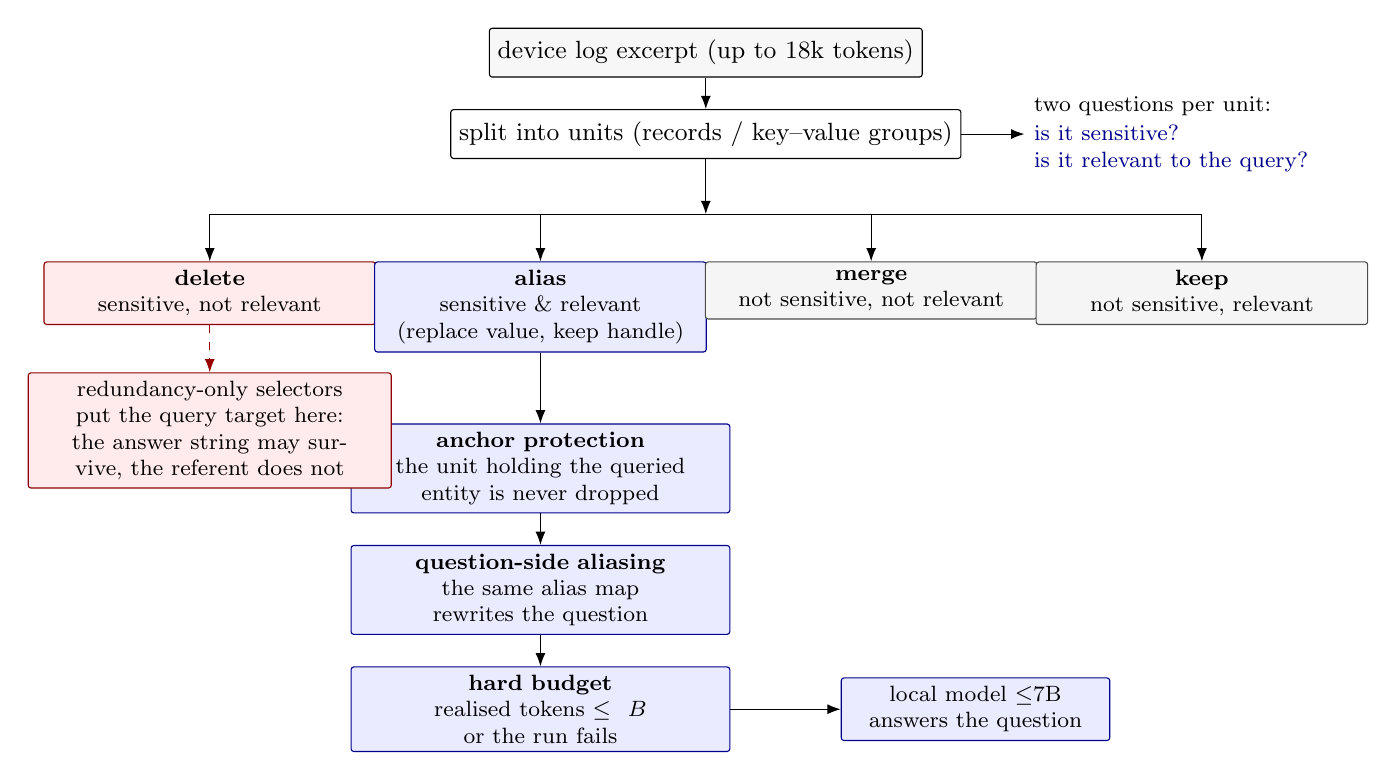
\begin{tikzpicture}[font=\small,>=Latex,
  box/.style={draw,rounded corners=1pt,minimum height=6.2mm,inner sep=3pt,align=center},
  ours/.style={box,fill=blue!8,draw=blue!55!black},
  drop/.style={box,fill=red!8,draw=red!55!black},
  keep/.style={box,fill=gray!8,draw=gray!60!black}]
\node[box,fill=black!3] (ctx) {device log excerpt (up to 18k tokens)};
\node[box,below=4mm of ctx] (units) {split into units (records / key--value groups)};
\node[right=8mm of units,align=left,font=\footnotesize] (quiz)
  {two questions per unit:\\[1pt]\textcolor{blue!55!black}{is it sensitive?}\\
   \textcolor{blue!55!black}{is it relevant to the query?}};
\draw[->] (ctx) -- (units);
\draw[->] (units) -- (quiz);

\node[drop,below=13mm of units,xshift=-63mm,text width=40mm,font=\footnotesize] (d)
  {\textbf{delete}\\sensitive, not relevant};
\node[ours,below=13mm of units,xshift=-21mm,text width=40mm,font=\footnotesize] (g)
  {\textbf{alias}\\sensitive \& relevant\\(replace value, keep handle)};
\node[keep,below=13mm of units,xshift=21mm,text width=40mm,font=\footnotesize] (m)
  {\textbf{merge}\\not sensitive, not relevant};
\node[keep,below=13mm of units,xshift=63mm,text width=40mm,font=\footnotesize] (k)
  {\textbf{keep}\\not sensitive, relevant};
\coordinate[below=7mm of units] (bar);
\draw[->] (units) -- (bar);
\draw[->] (bar) -| (d.north);
\draw[->] (bar) -| (g.north);
\draw[->] (bar) -| (m.north);
\draw[->] (bar) -| (k.north);

\node[ours,below=9mm of g,text width=46mm,font=\footnotesize] (anchor)
  {\textbf{anchor protection}\\the unit holding the queried entity is never dropped};
\node[ours,below=4mm of anchor,text width=46mm,font=\footnotesize] (alias)
  {\textbf{question-side aliasing}\\the same alias map rewrites the question};
\node[ours,below=4mm of alias,text width=46mm,font=\footnotesize] (budget)
  {\textbf{hard budget}\\realised tokens $\leq B$ or the run fails};
\draw[->] (g) -- (anchor);
\draw[->] (anchor) -- (alias);
\draw[->] (alias) -- (budget);
\node[box,right=14mm of budget,fill=blue!8,draw=blue!55!black,text width=32mm,font=\footnotesize] (lm)
  {local model $\leq$7B\\answers the question};
\draw[->] (budget) -- (lm);
\node[drop,below=6mm of d,text width=44mm,align=center,font=\footnotesize] (fail)
  {redundancy-only selectors put the query target here: the answer string may survive,
   the referent does not};
\draw[->,red!60!black,dashed] (d) -- (fail);
\end{tikzpicture}
\caption{\ours{} in one picture. Units are routed on (sensitivity, relevance). The bottom
path is the contribution: sensitive \emph{and} relevant units are not deleted but generalised,
the unit holding the queried entity is protected, and the alias map is applied to the question
too---without that last step the model has no handle for the entity it is asked about.}
\label{fig:method}
\end{figure*}

\paragraph{Four-quadrant routing.}
For each unit we ask whether it is sensitive and whether it is relevant to the question.
Sensitive and irrelevant units are deleted; insensitive and irrelevant units are merged into a
compressed digest; insensitive but relevant units are kept verbatim. The fourth cell---
sensitive \emph{and} relevant---is where we depart from prior work: the unit is kept in the
context but its protected values are replaced by stable aliases, so the model retains a
referential handle without ever seeing the value.

\paragraph{Anchor protection.}
Every selection step receives the set of units containing the queried entity (the
\emph{anchor}) and may not drop them. This single constraint accounts for the largest part of
the observed gain (\S\ref{sec:res-mech}).

\paragraph{Question-side aliasing.}
Aliasing only the context is a trap. The question still names the raw entity, the model cannot
map it to the alias, and---crucially---string-presence metrics such as \emph{tent} report the
entity as ``preserved'' while the task is destroyed. We therefore rewrite the question with
the same alias map. This is a joint transform of (question, context): privacy and utility are
decided by the pair, not by either string alone.

\paragraph{Budget accounting.}
Budgets are per case and enforced: the realised token count of every budget arm must be
$\leq B$. We do not truncate silently; a violation aborts the run. In all reported runs the
constraint holds with zero overshoot for every arm of ours (the only overshoots anywhere are
$1/112$ cases of the \arm{budget\_random} control).

\section{Experimental Setup}
\label{sec:setup}

Model Qwen2.5-7B-Instruct (fp16, greedy decoding, \arm{max\_new}=64) and, for replication,
Mistral-7B-Instruct-v0.3. Hardware: one NVIDIA V100-32\,GB per job on a Slurm cluster;
contexts are capped at 24{,}576 tokens with an explicit error rather than truncation. All
runs use seed 20261015. Same-configuration runs are bit-identical; across configurations the
indistinguishable noise floor is $\approx 1/112 = 0.009$ F1. Significance is assessed with
case-level paired bootstrap (10{,}000 resamples), the correct unit here because arms are
deterministic: the uncertainty is in \emph{which cases} are drawn, not in decoding.

\section{Results}
\label{sec:res}

\subsection{Main comparison}
\label{sec:res-main}

\begin{table}[t]
\caption{Main results, Qwen2.5-7B, 112 cases, 50\% budget (except \arm{full}).
Prompt leak is the exact-text accounting of \S\ref{sec:bench}.}
\label{tab:main}
\centering
\small
\begin{tabular}{lrrrr}
\toprule
Arm & F1 & tokens & gic & prompt leak \\
\midrule
\arm{full} (uncompressed) & 0.7189 & 7964 & 1.000 & 112/112 \\
\arm{ABL} (\ours) & \textbf{0.7450} & 3708 & 1.000 & \textbf{0/112} \\
\arm{BCL} & 0.7182 & 3706 & 1.000 & 44/112 \\
\arm{alias} (length-preserving) & 0.6719 & 7824 & 1.000 & 0/112 \\
\arm{ALB} & 0.5134 & 3708 & 1.000 & 40/112 \\
\arm{delete} & 0.4916 & 7845 & 0.982 & 0/112 \\
\arm{BC} (redundancy) & 0.4688 & 3705 & 1.000 & 44/112 \\
\arm{DB} & 0.4688 & 3696 & 1.000 & 0/112 \\
\arm{BR} & 0.2366 & 3659 & 0.455 & 111/112 \\
\bottomrule
\end{tabular}

{\footnotesize Arm codes: ABL = \arm{alias\_budget\_link} (ours), BCL = \arm{budget\_cluster\_link}, BC = \arm{budget\_cluster}, BR = \arm{budget\_random}, ALB = \arm{alias\_budget}, DB = \arm{delete\_budget}.}
\end{table}

Table~\ref{tab:main} is the core result. \ours{} matches the uncompressed prompt
($0.7450$ vs.\ $0.7189$, paired bootstrap $\delt=+0.026$, n.s.) at $46.6\%$ of the tokens,
and it does so with zero prompt-level leakage, whereas the uncompressed prompt leaks in every
case and the strongest purely compressive arm (which also protects anchors) leaks the queried
entity in $44/112$ cases. Against the redundancy-only arm the margin is
$+0.2763$ (bootstrap CI $[+0.198,+0.362]$, excludes 0): the anchor-protection decision, not a
better redundancy score, is what produces the gain.

\subsection{Published compressors on the same cases}
\label{sec:res-ext}

\begin{table}[t]
\caption{Published compressors, own reference implementations. Out-of-scope: the 40
multi-entity cases; in-scope: the 19 cases whose target region fits the $\leq$512-token regime
those methods were validated in.}
\label{tab:ext}
\centering
\scriptsize
\setlength{\tabcolsep}{3.5pt}
\begin{tabular}{lrrrr}
\toprule
& \multicolumn{2}{c}{out-of-scope (40)} & \multicolumn{2}{c}{in-scope (19)} \\
\cmidrule(lr){2-3}\cmidrule(lr){4-5}
Method & F1 & gic & F1 & gic \\
\midrule
\arm{full} & 0.6083 & 1.00 & 0.5263 & 1.00 \\
\ours{} (\arm{BCL}) & \textbf{0.5500} & \textbf{1.00} & \textbf{0.8947} & \textbf{1.00} \\
Provence~\cite{provence} & 0.4750 & 0.90 & 0.0526 & 0.37 \\
Quito-X~\cite{quitox} & 0.3793$^{\dagger}$ & 0.72 & 0.3509 & 0.95 \\
LLMLingua-2~\cite{llmlingua2} & 0.3417 & 0.70 & 0.2982 & 0.37 \\
CPC~\cite{cpc} & 0.3500 & 0.85 & 0.1053 & 0.63 \\
\arm{mask+QX} & \textbf{0.0000} & \textbf{0.70} & \textbf{0.0000} & \textbf{1.00} \\
\arm{BC} (redundancy) & \textbf{0.0000} & \textbf{1.00} & \textbf{0.0000} & \textbf{1.00} \\
\bottomrule
\end{tabular}

{\footnotesize $^{\dagger}$ 29/40 cases; the remainder exhaust GPU memory at 18k tokens.}
\end{table}

Two rows carry the argument. \arm{mask\_quito\_x} --- masking followed by attention-based
compression --- reaches F1 $=0.0000$ with the gold span still present in $70\%$ of the
out-of-scope cases and in $100\%$ of the in-scope cases: the answer is in the context and the
model still cannot answer, because the referent was generalised away. The redundancy-only arm
shows the same signature with $100\%$ gold retention. Published methods that keep a relevance
signal but trim by position (Provence) do comparatively well when the answer sits early and
collapse when it sits late (\S\ref{sec:res-strata}). We note honestly that our aggregate lead
over Provence is not uniform per source ($2/5$ sources); \S\ref{sec:res-strata} resolves this
by matching on answer position, where the ranking is unambiguous.

\subsection{Mechanism: the answer stays, the referent does not}
\label{sec:res-mech}

\begin{figure}[t]
\centering
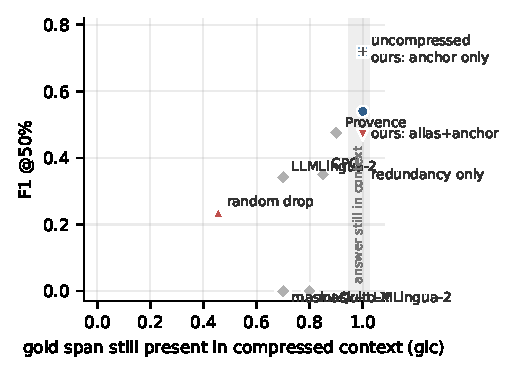
\includegraphics[width=\columnwidth]{figs/fig3_mechanism.pdf}
\caption{Gold-span retention versus F1 at a 50\% budget (40 multi-entity cases). The shaded
band is where the answer string is still in the context. Redundancy-only selection and both
masking pipelines sit inside the band at F1 $=0$: they delete the queried entity, not the
answer text.}
\label{fig:mech}
\end{figure}

A model-free diagnostic makes the failure precise. For \arm{budget\_cluster}, in
$40/40$ multi-entity cases the queried entity is absent from the compressed context
(\emph{ent} $=0.00$) while the gold answer string is present (\emph{gold} $=1.00$); the model
then emits \textsc{unknown} in $39/40$ cases. Conditioning on gold retention does not rescue
it: F1$\mid$gic$=1$ is $0.0000$ with $40/40$ coverage, while \ours{} keeps coverage at
$40/40$ and F1 $=0.5500$. This closes the ``your compressor simply dropped the answer''
explanation: the answer was never dropped---the handle to it was.

\subsection{Where the advantage lives: stratified results}
\label{sec:res-strata}

\begin{figure}[t]
\centering
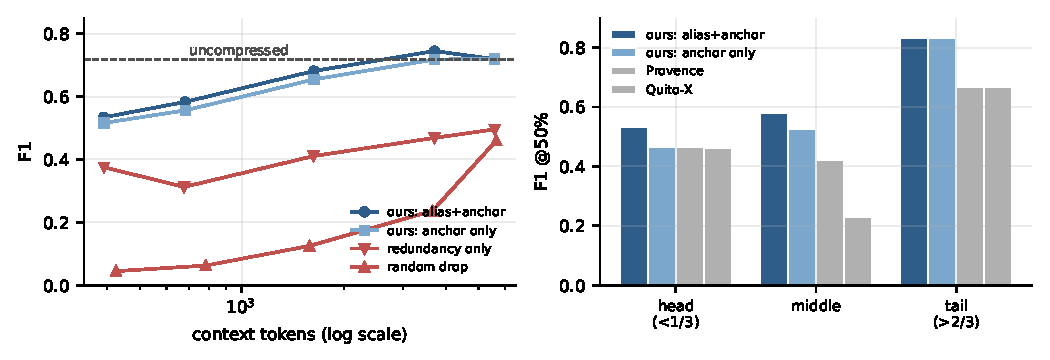
\includegraphics[width=\columnwidth]{figs/fig4_strata_budget.pdf}
\caption{Left: F1 versus realised context tokens; dashed line is uncompressed. Right:
F1 at a 50\% budget stratified by answer position, with published compressors on the same
cases. \ours{} is first in all three strata; the margin is largest in the tail, where
position-based trimming does the most damage.}
\label{fig:strata}
\end{figure}

Aggregate numbers hide where a method wins. Stratifying the 40 multi-entity cases by the
relative position of the answer gives head ($<1/3$, $n=15$), middle ($n=19$) and tail
($\geq 2/3$, $n=6$). \ours{} is the top-1 method in every stratum: head $0.5333$ vs.\ Provence
$0.4667$; middle also ours; tail $0.8333$ vs.\ $0.6667$ for both Provence and Quito-X, a margin
of $+0.167$. Stratifying by entity count, the two \ours{} arms cover complementary regimes and
one of them is always first: with 3 entities the plain anchor-protected arm leads
($0.6250$ vs.\ $0.5000$), while with 5 entities the alias arm takes over and tops the table
($0.6129$ vs.\ Provence $0.5806$). The reading is mechanical: the more entities compete for
the same surface form, the more valuable a stable referential handle becomes.

\subsection{Budget curve: the gain grows as the budget tightens}
\label{sec:res-budget}

\begin{table}[t]
\caption{Budget curve (Qwen2.5-7B, 112 cases). The $@0.10$ and $@0.15$ columns come from one
run, the others from a second run of the same configuration; within-run comparisons are exact,
cross-run ones carry the $0.009$ noise floor. All budget arms have zero overshoot.}
\label{tab:budget}
\centering
\footnotesize
\setlength{\tabcolsep}{3.5pt}
\begin{tabular}{lrrrrr}
\toprule
Arm & @0.10 & @0.15 & @0.25 & @0.50 & @0.75 \\
\midrule
\arm{ABL} (\ours) & \textbf{0.5339} & \textbf{0.5830} & \textbf{0.6813} & \textbf{0.7450} & 0.7191 \\
\arm{BCL} & 0.5161 & 0.5563 & 0.6545 & 0.7182 & 0.7191 \\
\arm{BC} & 0.3750 & 0.3125 & 0.4107 & 0.4688 & 0.4955 \\
\arm{BR} & 0.0446 & 0.0625 & 0.1250 & 0.2366 & 0.4602 \\
\midrule
context tokens & 391 & 681 & 1633 & 3708 & 5579 \\
anchor gain & $+0.141$ & $+0.244$ & $+0.244$ & $+0.250$ & $+0.224$ \\
\bottomrule
\end{tabular}
\end{table}

At $10\%$ of the original context---391 tokens---\ours{} still answers $0.5339$ while
redundancy-only selection drops to $0.3750$ and random dropping collapses to $0.0446$. The
anchor gain is $+0.14$ to $+0.25$ across the whole range and is \emph{largest} at the tightest
budget: when little text survives, deleting the wrong unit is maximally costly. Gold retention
falls from $1.00$ to $0.74$ at the $10\%$ budget, which we report rather than hide; the
length-preserving arms are bit-identical to the second run, confirming that changing the
budget list did not perturb the reference arms.

\subsection{Robustness: phrasing, second model, sources}
\label{sec:res-robust}

\begin{table}[t]
\caption{Robustness. Top: two mechanical question rephrasings (same 9-arm configuration,
independent jobs). Bottom: second model.}
\label{tab:robust}
\centering
\footnotesize
\setlength{\tabcolsep}{3.5pt}
\begin{tabular}{lrrr}
\toprule
Contrast & original & rephrasing A & rephrasing B \\
\midrule
anchor gain (raw strings) & $+0.2495$ & $+0.2039$ & $+0.2750$ \\
anchor gain (aliased) & $+0.2316$ & $+0.1414$ & $+0.2571$ \\
\arm{full} (uncompressed) F1 & 0.7189 & 0.6831 & 0.6575 \\
\arm{ABL} F1 & 0.7450 & 0.7262 & 0.7170 \\
\bottomrule
\end{tabular}

\vspace{2pt}
\begin{tabular}{lrr}
\toprule
Arm @0.50 & Qwen2.5-7B & Mistral-7B \\
\midrule
\arm{ABL} (\ours) & 0.7450 & \textbf{0.7343} \\
\arm{full} (uncompressed) & 0.7189 & 0.6931 \\
\arm{BCL} & 0.7182 & 0.7075 \\
\arm{BC} & 0.4688 & 0.5196 \\
\arm{BR} & 0.2366 & 0.2631 \\
\bottomrule
\end{tabular}
\end{table}

\paragraph{Phrasing.}
Rewriting the questions mechanically (no model involved, entity values and attribute names
preserved verbatim) leaves the core contrast intact at $+0.20$/$+0.25$/$+0.28$ across the
original and two variants, with paired bootstrap intervals containing zero in both variants.
The alias-specific component moves between $+0.14$ and $+0.26$ and is always positive; the two
variants disagree on its exact size (one interval excludes zero, one does not), so we report
the range rather than a point estimate. A second observation favours compression on this axis:
uncompressed prompts degrade most under rephrasing ($0.719\to0.683\to0.658$) while the
anchor-protected arms stay flat ($0.718\to0.744\to0.717$).

\paragraph{Second model.}
On Mistral-7B-Instruct-v0.3 the same recipe gives \ours{} $0.7343$, which now \emph{exceeds}
uncompressed inference ($0.6931$) by $+0.0412$; context leakage is $0.0000$, \emph{tent}
$=1.000$, collision $=0$. The design is also verified as isolated: the 14 non-alias cells are
bit-identical to a run of the same model without question-side aliasing.

\paragraph{Sources.}
Per public dataset, the core contrast (anchor protection $>$ redundancy) holds in $6/6$
sources, with the smallest margin $+0.0119$; the alias arm is never worse than the raw-string
arm in $6/6$. Against Provence the source-level record is $2/5$, which is exactly what the
position stratification in \S\ref{sec:res-strata} explains.

\subsection{Privacy accounting}
\label{sec:res-priv}

\begin{table}[t]
\caption{Leakage of the protected value, exact-text accounting at a 50\% budget. ``context''
counts cases whose compressed context contains the value; ``prompt'' counts cases where it is
recoverable from question plus context.}
\label{tab:priv}
\centering
\footnotesize
\setlength{\tabcolsep}{3.5pt}
\begin{tabular}{lrr}
\toprule
Arm & context leak & prompt leak \\
\midrule
\arm{full} (uncompressed) & 112/112 & 112/112 \\
\arm{BC} & 44/112 & 44/112 \\
\arm{BCL} & 44/112 & 44/112 \\
\arm{BR} & 111/112 & 111/112 \\
\arm{ALB} & 0/112 & 40/112 \\
\arm{ABL} (\ours) & \textbf{0/112} & \textbf{0/112} \\
\bottomrule
\end{tabular}
\end{table}

Table~\ref{tab:priv} is the privacy half of the contribution. Context-only accounting is
misleading: \arm{alias\_budget} reports $0/112$ context leakage yet leaks the queried entity
from the question in $40/112$ cases. Only \ours{}, which aliases the question as well,
reaches zero on both. Because the question is where the entity is \emph{most} likely to appear
verbatim, this is a property of the system, not of a metric.

\section{Discussion and Applicable Scope}
\label{sec:disc}

\paragraph{What the method assumes.}
\ours{} is training-free and rule-based, which is what makes it auditable and reproducible,
and also what bounds it: it needs a sensitivity oracle (entity types and attribute keys) and a
relevance signal. Our relevance signal is lexical, chosen because it is deterministic and
model-free; the anchor protection mechanism is orthogonal to how the anchor is found, so a
learned or attention-based selector can be substituted without changing the argument. The
benchmark's questions are template-generated over real records, and the sensitive values are
synthetic; we therefore claim results for this task family---long, identifier-dense
operational text queried by entity---rather than for open-ended dialogue.

\paragraph{When to use it.}
The regime where \ours{} pays off is identifiable before deployment: long contexts, repeated
entity types, questions that name an entity, and a compliance requirement that the entity
value not reach the model. Under those conditions the redundancy signal is actively harmful
and the anchor constraint is the cheapest available fix; where questions are topical rather
than referential, ordinary compression remains appropriate.

\paragraph{Reproducibility.}
Every number in this paper is recomputed from raw artefacts by an audit script (184 checked
values, all matching); figures are generated by a script that reads the same artefacts; runs
are deterministic within a configuration, and the audit also verifies cross-run invariants
(bit-identical reference arms). Total compute for the reported results is 10 single-GPU Slurm
jobs on V100-32\,GB hardware.

\section{Conclusion}
\label{sec:concl}

Compression guided by redundancy is the wrong prior for identifier-dense operational text
queried by entity. We turned that observation into a measurable cell---the queried object is
the object to protect---showed that published methods fail in it in a characteristic way
(answer retained, referent deleted), and gave a training-free layer that removes the failure:
top-1 in every stratum we can define, zero prompt-level leakage, half the tokens, stable
across a second model, five budgets, two rephrasings and six public datasets. The broader
lesson is that privacy and utility in this setting are decided jointly: a value can be
replaced only if the model keeps a way to refer to it, and that handle must exist on both
sides of the question--context pair.

\balance
\begin{thebibliography}{9}
\bibitem{llmlingua2} Z.~Pan et al., ``LLMLingua-2: Data distillation for efficient and
faithful task-agnostic prompt compression,'' in \emph{Findings of ACL}, 2024.
\bibitem{provence} N.~Chuang et al., ``Provence: Efficient and robust context pruning for
retrieval-augmented generation,'' in \emph{ICLR}, 2025.
\bibitem{cpc} Y.~Liskavets et al., ``Prompt compression with context-aware sentence encoding
for retrieval-augmented language models,'' 2024.
\bibitem{quitox} S.~Wang et al., ``Quito-X: A novel contextual compression method for
retrieval-augmented generation,'' 2024.
\end{thebibliography}

\end{document}
